%----------------------------------------------------------------------------------------
% RIJEN: BEGRIPPEN. Alle opgaven zijn eigen werk.
%
% Opbouw: Start, leerstof (kern, uitgewerkt voorbeeld, korte oefening), en daarna op een
% nieuwe pagina de Opdrachten (door elkaar, stijgende moeilijkheid), Koppel en Test jezelf.
% Labels van dit hoofdstuk beginnen met h1-.
%----------------------------------------------------------------------------------------

% Kleine grafiek van een rij: {naam}{ymin}{ymax}{ticks op de y-as}{punten n/u_n}
\newcommand{\minigrafiek}[5]{%
  \pgfmathsetmacro{\eenheid}{2.3/(#3-(#2))}%
  \begin{tikzpicture}[x=.38cm,y=\eenheid cm,>={Stealth[length=1.4mm]},font=\scriptsize]
    \draw[->,lijngrijs] (-.2,0) -- (6.8,0) node[right,text=black] {$n$};
    \draw[->,lijngrijs] (0,#2) -- (0,#3) node[above,text=black] {$u_n$};
    \foreach \x in {1,...,6} \draw[lijngrijs] (\x,0) ++(0,1.2pt) -- ++(0,-2.4pt) node[below=-1pt,text=grijs] {\x};
    \foreach \y in {#4} \draw[lijngrijs] (0,\y) ++(1.2pt,0) -- ++(-2.4pt,0) node[left=-1pt,text=grijs] {$\y$};
    \foreach \x/\y in {#5} \fill[accent] (\x,\y) circle (1.6pt);
    \node[anchor=south,font=\sffamily\bfseries\footnotesize] at (3.4,#3) {#1};
  \end{tikzpicture}}

\mychapter{1}{Rijen: begrippen}

\lkr{Leerplan B+S'': LPD 44 (recursief en expliciet voorschrift, rij als discrete functie). Dit hoofdstuk legt de begrippen vast voor hoofdstuk 2; rekenkundige en meetkundige rijen krijgen hier nog geen naam. Drie rode draden: het verschil tussen volgnummer en term, het verschil tussen expliciet en recursief, en de grafiek met losse punten.}

\begin{oefeningen}[Start]
\begin{oefening}
\blokkop{Opwarmer}
\begin{enumerate}
  \item Gegeven: $f(x) = x^2 - 3x$. Bereken $f(4)$ en $f(-1)$.
  \item Bereken $(-1)^5$, $(-1)^{12}$, $-2^4$ en $(-2)^4$.
  \item Werk uit en vereenvoudig: $(n+1)^2 - n^2$.
  \item Los op: $n^2 + n - 12 = 0$.
  \item Bepaal het domein van $f(x) = \dfrac{3}{x-2}$.
\end{enumerate}
\begin{solution}
\textbf{a.}~4 en 4 \quad \textbf{b.}~$-1$; 1; $-16$; 16 \quad \textbf{c.}~$2n+1$ \quad \textbf{d.}~$n=3$ of $n=-4$ \quad \textbf{e.}~$\mathbb{R}\setminus\{2\}$
\end{solution}
\begin{fullsolution}
\textbf{a.}~$f(4)=16-12=4$ en $f(-1)=1+3=4$.\\
\textbf{b.}~Oneven exponent: $(-1)^5=-1$. Even exponent: $(-1)^{12}=1$. Zonder haakjes hoort de macht alleen bij 2: $-2^4=-16$. Met haakjes: $(-2)^4=16$.\\
\textbf{c.}~$n^2+2n+1-n^2=2n+1$.\\
\textbf{d.}~$(n-3)(n+4)=0$, dus $n=3$ of $n=-4$.\\
\textbf{e.}~De noemer mag niet nul zijn, dus $x\neq 2$.
\end{fullsolution}
\end{oefening}

\begin{oefening}\label{oef:h1-verken}
\blokkop{Verken}\quad Met blokjes bouw je trappen. Trap 1 telt 1 blokje, trap 2 telt 3 blokjes, trap 3 telt 6 blokjes.

\begin{tikzpicture}[x=3.1mm,y=3.1mm]
  \foreach \n/\s in {1/0,2/3,3/7,4/12}{
    \foreach \k in {1,...,\n}{
      \foreach \h in {1,...,\k}{
        \draw[accent,fill=accent!15] (\s+\k-1,\h-1) rectangle ++(1,1);}}
    \node[below,font=\scriptsize\sffamily] at (\s+\n/2,0) {trap \n};}
\end{tikzpicture}
\begin{enumerate}
  \item Hoeveel blokjes telt trap 4? En trap 5?
  \item Trap 9 telt 45 blokjes. Hoeveel blokjes telt trap 10? Hoe zie je dat zonder te tekenen?
  \item Leg twee gelijke trappen tegen elkaar, één ervan omgekeerd. Welke rechthoek krijg je met twee keer trap 4? Hoeveel blokjes telt trap 100 dan?
\end{enumerate}
\begin{solution}
\textbf{a.}~10 en 15 \quad \textbf{b.}~55 \quad \textbf{c.}~4 op 5; 5050
\end{solution}
\begin{fullsolution}
\textbf{a.}~Er komt telkens een kolom bij: $6+4=10$ en $10+5=15$.\\
\textbf{b.}~Trap 10 is trap 9 plus een kolom van 10 blokjes: $45+10=55$.\\
\textbf{c.}~Twee keer trap 4 geeft een rechthoek van 4 op 5, dus trap 4 telt $\dfrac{4\cdot 5}{2}=10$ blokjes. Zo telt trap 100 er $\dfrac{100\cdot 101}{2}=5050$.
\end{fullsolution}
\end{oefening}
\end{oefeningen}

\lkr{Laat oefening \ref{oef:h1-verken} maken vóór de uitleg. In b redeneren leerlingen recursief (de vorige trap plus een kolom), in c expliciet (rechtstreeks uit het nummer van de trap). Kom hierop terug bij de theorie \emph{Expliciet of recursief?}.}

%========================================================================================
\section{Termen en volgnummers}

\begin{theorie}
Een \emph{rij} is een opeenvolging van getallen in een vaste volgorde. De getallen zijn de \emph{termen} van de rij. De index is het \emph{volgnummer}: $u_1$ is de eerste term, $u_2$ de tweede, en $u_n$ de $n$-de term of \emph{algemene term}, met $n \in \mathbb{N}_0$.

\vspace{1mm}
{\renewcommand{\arraystretch}{1.25}%
\begin{tabular}{@{}l*{7}{>{\centering\arraybackslash}p{11mm}}@{}}
volgnummer & 1 & 2 & 3 & $\cdots$ & $n-1$ & $n$ & $n+1$ \\
term & $u_1$ & $u_2$ & $u_3$ & $\cdots$ & $u_{n-1}$ & $u_n$ & $u_{n+1}$
\end{tabular}}

\vspace{1mm}
Let op: $u_{n-1}$ is de term vóór $u_n$. Dat is iets anders dan $u_n - 1$.
\end{theorie}

\thuis{Het volgnummer zegt \emph{waar} een term staat, de term zelf zegt \emph{welk getal} daar staat. In de rij $7,\ 2,\ 9,\ \ldots$ is $u_3 = 9$: op plaats 3 staat het getal 9. Drie puntjes betekenen dat de rij verdergaat.}

\voorbeeld{}{Het aantal dagen per maand in een gewoon jaar geeft een rij:\\[.5ex]
$31,\ 28,\ 31,\ 30,\ 31,\ 30,\ 31,\ 31,\ 30,\ 31,\ 30,\ 31$\\[.5ex]
Geef $u_2$ en $u_7$. Voor welke volgnummers is $u_n = 30$?\label{vb:h1-maanden}}{%
\begin{stappen}
u_2 = 28 & De tweede term: februari. \\
u_7 = 31 & De zevende term: juli. \\
n = 4,\ 6,\ 9 \text{ of } 11 & Eenzelfde getal mag meer dan eens voorkomen. Bij een volgnummer hoort wel maar één term.
\end{stappen}}

\lkr{Deze rij heeft twaalf termen en geen handig voorschrift. Zo zien leerlingen meteen dat een rij meer is dan een formule.}

\nujij{In de rij $4,\ 7,\ 7,\ 1,\ 0,\ 7$: wat is $u_3$? Voor welke volgnummers is $u_n = 7$?}{$u_3 = 7$; $n = 2$, 3 of 6.}

\begin{oefeningen}
\begin{oefening}
Gegeven is de rij $8,\ 3,\ 8,\ 0,\ 5,\ 3,\ 1$.
\begin{enumerate}
  \item Wat is $u_4$?
  \item Voor welke volgnummers is $u_n = 3$?
  \item Neem $n = 5$. Wat zijn $u_{n-1}$ en $u_{n+1}$?
\end{enumerate}
\begin{solution}
\textbf{a.}~0 \quad \textbf{b.}~$n=2$ of $n=6$ \quad \textbf{c.}~0 en 3
\end{solution}
\begin{fullsolution}
\textbf{a.}~De vierde term is 0.\\
\textbf{b.}~Het getal 3 staat op plaats 2 en plaats 6.\\
\textbf{c.}~$u_{n-1}=u_4=0$ en $u_{n+1}=u_6=3$.
\end{fullsolution}
\end{oefening}
\end{oefeningen}

%========================================================================================
\section{Expliciet voorschrift}

\subsection{Termen berekenen}

\begin{theorie}
Een \emph{expliciet voorschrift} geeft $u_n$ rechtstreeks uit het volgnummer $n$. Je kunt elke term berekenen zonder de vorige termen te kennen.
\end{theorie}

\voorbeeld{}{Gegeven: $u_n = n^2 - 5n + 7$. Bereken $u_1$, $u_2$, $u_3$ en $u_{10}$. Schrijf ook $u_{n+1}$ zo eenvoudig mogelijk.\label{vb:h1-termen}}{%
\begin{stappen}
u_1 = 1 - 5 + 7 = 3 & Vervang $n$ door 1. \\
u_2 = 4 - 10 + 7 = 1, \quad u_3 = 9 - 15 + 7 = 1 & Twee termen kunnen gelijk zijn. \\
u_{10} = 100 - 50 + 7 = 57 & De vorige termen heb je niet nodig. \\
u_{n+1} = (n+1)^2 - 5(n+1) + 7 & Vervang $n$ door $n+1$, met haakjes. \\
\phantom{u_{n+1}} = n^2 - 3n + 3 & Dit is de volgende term, en dus niet $u_n + 1$.
\end{stappen}}

\lkr{Laat leerlingen $u_{n+1}$ en $u_n + 1$ naast elkaar uitrekenen voor $n = 2$: 1 en 2. De indexnotatie is voor veel leerlingen het eerste struikelblok.}

\nujij{Gegeven: $u_n = 3n - n^2$. Bereken $u_1$, $u_4$ en $u_{n-1}$.}{$u_1 = 2$; $u_4 = -4$; $u_{n-1} = 3(n-1) - (n-1)^2 = -n^2 + 5n - 4$.}

\begin{oefeningen}
\begin{oefening}
Gegeven: $u_n = 2n^2 - n$. Bereken $u_1$, $u_2$, $u_3$ en $u_{20}$. Schrijf ook $u_{n-1}$ zo eenvoudig mogelijk.
\begin{solution}
1; 6; 15; 780; $u_{n-1}=2n^2-5n+3$
\end{solution}
\begin{fullsolution}
$u_1=2-1=1$, $u_2=8-2=6$, $u_3=18-3=15$, $u_{20}=800-20=780$.\\
$u_{n-1}=2(n-1)^2-(n-1)=2n^2-4n+2-n+1=2n^2-5n+3$.
\end{fullsolution}
\end{oefening}
\end{oefeningen}

\subsection{Voorschrift opstellen}

\begin{werkwijze}
Zoek het verband tussen volgnummer en term.
\begin{itemize}
  \item Vergelijk de termen met $n$, met $n^2$ en met machten zoals $2^n$. Tel er zo nodig iets bij of trek er iets van af.
  \item Bij een breuk bekijk je teller en noemer apart.
  \item Wisselend teken: $(-1)^n$ geeft $-1,\ 1,\ {-1},\ 1,\ \ldots$ en $(-1)^{n+1}$ geeft $1,\ {-1},\ 1,\ {-1},\ \ldots$
  \item Controleer je voorschrift met een term die je nog niet gebruikt hebt.
\end{itemize}
\end{werkwijze}

\voorbeeld{}{Bepaal een expliciet voorschrift van $\tfrac13,\ {-\tfrac25},\ \tfrac37,\ {-\tfrac49},\ \ldots$\label{vb:h1-opstellen}}{%
\begin{stappen}
\text{teken: } (-1)^{n+1} & Positief bij oneven $n$, negatief bij even $n$. \\
\text{teller: } 1,\ 2,\ 3,\ 4 \ \Rightarrow \ n & De teller is het volgnummer. \\
\text{noemer: } 3,\ 5,\ 7,\ 9 \ \Rightarrow \ 2n+1 & Telkens 2 meer: het dubbele van $n$, plus 1. \\[1ex]
u_n = (-1)^{n+1} \cdot \dfrac{n}{2n+1} & Controle: $u_4 = (-1)^5 \cdot \dfrac{4}{9} = -\dfrac{4}{9}$.
\end{stappen}}

\thuis{\blokkop{Half uitgewerkt}\quad Rij $3,\ 6,\ 11,\ 18,\ \ldots$ Vergelijk met de kwadraten $1,\ 4,\ 9,\ 16$. Schrijf over in je schrift en vul aan: \ elke term is $\vak$ meer dan $n^2$, dus $u_n = \vak$ en $u_5 = \vak$. \quad {\footnotesize(Antwoord: 2 meer, $u_n = n^2 + 2$ en $u_5 = 27$.)}}

\nujij{Bepaal een expliciet voorschrift van $1,\ {-\tfrac12},\ \tfrac13,\ {-\tfrac14},\ \ldots$}{$u_n = (-1)^{n+1} \cdot \tfrac1n$.}

\begin{oefeningen}
\begin{oefening}
Bepaal een expliciet voorschrift.
\begin{reeks}
  \item $6,\ 11,\ 16,\ 21,\ \ldots$
  \item $2,\ 5,\ 10,\ 17,\ \ldots$
  \item $-\tfrac12,\ \tfrac23,\ {-\tfrac34},\ \tfrac45,\ \ldots$
\end{reeks}
\begin{solution}
\textbf{a.}~$u_n=5n+1$ \quad \textbf{b.}~$u_n=n^2+1$ \quad \textbf{c.}~$u_n=(-1)^n\cdot\dfrac{n}{n+1}$
\end{solution}
\begin{fullsolution}
\textbf{a.}~Telkens 5 meer, dus vergelijk met $5n$: $5,\ 10,\ 15$. Elke term is 1 meer: $u_n=5n+1$.\\
\textbf{b.}~Elke term is 1 meer dan een kwadraat: $u_n=n^2+1$.\\
\textbf{c.}~Negatief bij oneven $n$, teller $n$, noemer $n+1$: $u_n=(-1)^n\cdot\dfrac{n}{n+1}$.
\end{fullsolution}
\end{oefening}
\end{oefeningen}

\subsection{Term of geen term}

\begin{werkwijze}
Is $x$ een term van de rij? Los $u_n = x$ op. Is er een oplossing $n \in \mathbb{N}_0$, dan is $x$ de $n$-de term. Anders is $x$ geen term.
\end{werkwijze}

\voorbeeld{}{Gegeven: $u_n = n^2 + 2n$. Is 48 een term van de rij? En 50?\label{vb:h1-isterm}}{%
\begin{stappen}
n^2 + 2n - 48 = 0 \ \Rightarrow \ (n-6)(n+8) = 0 & $n = 6$ of $n = -8$. Enkel $n = 6$ is een volgnummer: \textbf{ja}, 48 is de 6de term. \\
n^2 + 2n - 50 = 0 \ \Rightarrow \ n = -1 \pm \sqrt{51} & $n \approx 6{,}14$ of $n \approx -8{,}14$. Geen volgnummer: \textbf{nee}.
\end{stappen}}

\nujij{Gegeven: $u_n = n^2 + n$. Is 90 een term van de rij? En 100?}{90 is de 9de term ($n = 9$ of $n = -10$). Bij 100 is $n \approx 9{,}51$, dus geen term.}

\begin{oefeningen}
\begin{oefening}
Gegeven: $u_n = n^2 - 4n$. Is 21 een term van de rij? En 20?
\begin{solution}
21 is de 7de term; 20 is geen term.
\end{solution}
\begin{fullsolution}
$n^2-4n-21=0$ geeft $(n-7)(n+3)=0$, dus $n=7$ (en $n=-3$ valt weg).\\
$n^2-4n-20=0$ geeft $n=2\pm\sqrt{24}$, dus $n\approx 6{,}90$ of $n\approx -2{,}90$: geen volgnummer.
\end{fullsolution}
\end{oefening}
\end{oefeningen}

\subsection{Starten bij volgnummer 0}

Bij iets dat in de tijd verandert, start je vaak bij $u_0$: de beginwaarde, voor er een stap gebeurd is. Dan is $u_n$ de waarde na $n$ stappen, en is $u_1$ de \emph{tweede} term.

\voorbeeld{}{Een lift stijgt: de hoogte in meter is elke seconde $12,\ 15,\ 18,\ \ldots$ Geef een expliciet voorschrift als de eerste term $u_1$ heet, en als hij $u_0$ heet. Welk volgnummer heeft de hoogte 30 in elk geval?\label{vb:h1-nul}}{%
\begin{stappen}
u_1 = 12: \quad u_n = 3n + 9 & Controle: $3 \cdot 1 + 9 = 12$. \\
u_0 = 12: \quad u_n = 3n + 12 & Controle: $3 \cdot 0 + 12 = 12$. \\
3n + 9 = 30 \ \Rightarrow \ n = 7 & Bij start $u_1$ is 30 de term $u_7$. \\
3n + 12 = 30 \ \Rightarrow \ n = 6 & Bij start $u_0$ is 30 de term $u_6$: de hoogte na 6 seconden.
\end{stappen}}

\lkr{Hetzelfde getal, een ander volgnummer. In hoofdstuk 2 komt dit terug bij lineaire en exponentiële groei.}

\begin{oefeningen}
\begin{oefening}
Een vijver telt bij het begin 40 kikkers. $u_n$ is het aantal kikkers na $n$ jaar. Na een jaar zijn er 52, na twee jaar 61.
\begin{enumerate}
  \item Wat is $u_0$? Wat is $u_2$?
  \item Hoeveel termen tel je van $u_0$ tot en met $u_{10}$?
\end{enumerate}
\begin{solution}
\textbf{a.}~$u_0=40$ en $u_2=61$ \quad \textbf{b.}~11
\end{solution}
\begin{fullsolution}
\textbf{a.}~$u_0$ is het begin: 40. $u_2$ is het aantal na twee jaar: 61.\\
\textbf{b.}~De termen $u_1$ tot en met $u_{10}$ zijn er 10, en $u_0$ komt erbij: 11.
\end{fullsolution}
\end{oefening}
\end{oefeningen}

%========================================================================================
\section{Recursief voorschrift}

\subsection{Termen berekenen}

\begin{theorie}
Een \emph{recursief voorschrift} geeft $u_n$ uit een of meer vorige termen. Je hebt ook de \emph{begintermen} nodig: zonder die ligt de rij niet vast.
\end{theorie}

Bijvoorbeeld: $u_1 = 3$ en $u_n = 2u_{n-1} - 1$ voor $n \geqslant 2$. Hetzelfde voorschrift, met de index een plaats verschoven: $u_{n+1} = 2u_n - 1$ voor $n \geqslant 1$.

\thuis{\emph{Recursief} komt van het Latijnse \emph{recurrere}, teruglopen: je grijpt telkens terug naar de vorige term. Lees $u_n = 2u_{n-1} - 1$ dus als: een term is het dubbele van de vorige term, min 1.}

\voorbeeld{}{Gegeven: $u_1 = 3$ en $u_n = 2u_{n-1} - 1$ voor $n \geqslant 2$. Bereken $u_2$, $u_3$ en $u_4$.\label{vb:h1-rec}}{%
\begin{stappen}
u_2 = 2u_1 - 1 = 2 \cdot 3 - 1 = 5 & Vervang $n$ door 2: de vorige term is $u_1$. \\
u_3 = 2u_2 - 1 = 2 \cdot 5 - 1 = 9 & Elke stap gebruikt de uitkomst van de vorige stap. \\
u_4 = 2u_3 - 1 = 2 \cdot 9 - 1 = 17 & Voor $u_{100}$ moet je zo 99 stappen zetten.
\end{stappen}}

\nujij{Gegeven: $u_1 = 10$ en $u_n = u_{n-1} - 2n$ voor $n \geqslant 2$. Bereken $u_2$, $u_3$ en $u_4$.}{$u_2 = 6$; $u_3 = 0$; $u_4 = -8$.}

\begin{oefeningen}
\begin{oefening}
Gegeven: $u_1 = 1$ en $u_n = 3u_{n-1} + 2$ voor $n \geqslant 2$. Bereken $u_2$, $u_3$ en $u_4$.
\begin{solution}
5; 17; 53
\end{solution}
\begin{fullsolution}
$u_2=3\cdot 1+2=5$, $u_3=3\cdot 5+2=17$, $u_4=3\cdot 17+2=53$.
\end{fullsolution}
\end{oefening}
\end{oefeningen}

\subsection{Twee begintermen}

Gebruikt het voorschrift twee vorige termen, dan heb je twee begintermen nodig. De bekendste is de \emph{rij van Fibonacci}: $u_1 = u_2 = 1$ en $u_n = u_{n-1} + u_{n-2}$ voor $n \geqslant 3$. Die geeft $1,\ 1,\ 2,\ 3,\ 5,\ 8,\ 13,\ \ldots$

\voorbeeld{}{Gegeven: $u_1 = 2$, $u_2 = 3$ en $u_n = u_{n-1} \cdot u_{n-2} - 1$ voor $n \geqslant 3$. Bereken $u_3$, $u_4$ en $u_5$.\label{vb:h1-twee}}{%
\begin{stappen}
u_3 = u_2 \cdot u_1 - 1 = 3 \cdot 2 - 1 = 5 & Bij $n = 3$ zijn de twee vorige termen $u_2$ en $u_1$. \\
u_4 = u_3 \cdot u_2 - 1 = 5 \cdot 3 - 1 = 14 & \\
u_5 = u_4 \cdot u_3 - 1 = 14 \cdot 5 - 1 = 69 &
\end{stappen}}

\begin{oefeningen}
\begin{oefening}
Bepaal de eerste vijf termen.
\begin{enumerate}
  \item $u_1 = 5$, $u_2 = 2$ en $u_n = u_{n-1} + u_{n-2}$ voor $n \geqslant 3$
  \item $u_1 = 1$ en $u_n = u_{n-1} + 2n$ voor $n \geqslant 2$
\end{enumerate}
\begin{solution}
\textbf{a.}~5, 2, 7, 9, 16 \quad \textbf{b.}~1, 5, 11, 19, 29
\end{solution}
\begin{fullsolution}
\textbf{a.}~$u_3=2+5=7$, $u_4=7+2=9$, $u_5=9+7=16$.\\
\textbf{b.}~$u_2=1+4=5$, $u_3=5+6=11$, $u_4=11+8=19$, $u_5=19+10=29$. Het volgnummer staat hier mee in het voorschrift.
\end{fullsolution}
\end{oefening}
\end{oefeningen}

\subsection{Voorschrift opstellen}

\begin{werkwijze}
Kijk hoe je van een term naar de volgende gaat: wat komt erbij, waarmee vermenigvuldig je? Hangt de stap af van het volgnummer, schrijf ze dan met $n$ en controleer ze bij de eerste stap. Vergeet de begintermen niet.
\end{werkwijze}

\voorbeeld{}{Bepaal een recursief voorschrift van $1,\ 2,\ 4,\ 7,\ 11,\ 16,\ \ldots$\label{vb:h1-recopst}}{%
\begin{stappen}
\text{erbij: } 1,\ 2,\ 3,\ 4,\ 5 & De stap wordt telkens 1 groter. \\
u_2 - u_1 = 1,\quad u_3 - u_2 = 2 & Van $u_{n-1}$ naar $u_n$ komt er dus $n - 1$ bij, en niet $n$. \\
u_n = u_{n-1} + (n-1),\ u_1 = 1 & Geldig voor $n \geqslant 2$. Controle: $u_5 = 7 + 4 = 11$.
\end{stappen}}

\lkr{De fout $u_n = u_{n-1} + n$ is hier heel gewoon. Laat leerlingen die fout zelf ontdekken door de eerste stap te controleren: dan is $u_2 = 3$.}

\begin{oefeningen}
\begin{oefening}
Bepaal een recursief voorschrift.
\begin{reeks}
  \item $3,\ 6,\ 12,\ 24,\ \ldots$
  \item $2,\ 3,\ 5,\ 8,\ 12,\ \ldots$
  \item $1,\ 4,\ 13,\ 40,\ \ldots$
\end{reeks}
\begin{solution}
\textbf{a.}~$u_n=2u_{n-1}$, $u_1=3$ \quad \textbf{b.}~$u_n=u_{n-1}+(n-1)$, $u_1=2$ \quad \textbf{c.}~$u_n=3u_{n-1}+1$, $u_1=1$
\end{solution}
\begin{fullsolution}
\textbf{a.}~Telkens maal 2.\\
\textbf{b.}~Er komt 1, 2, 3, 4 bij: bij de stap naar $u_n$ is dat $n-1$.\\
\textbf{c.}~Probeer een vermenigvuldiging: $3\cdot 1+1=4$, $3\cdot 4+1=13$, $3\cdot 13+1=40$.
\end{fullsolution}
\end{oefening}
\end{oefeningen}

\subsection{Expliciet of recursief?}

\begin{tabular}{@{}>{\RaggedRight\arraybackslash}p{7cm}>{\RaggedRight\arraybackslash}p{7.6cm}@{}}
\textbf{Expliciet:} rechtstreeks uit het volgnummer. Handig om meteen een verre term te berekenen. & \textbf{Recursief:} stap per stap uit de vorige termen. Handig om te beschrijven hoe een rij ontstaat. \\[2mm]
\begin{tikzpicture}[>={Stealth[length=1.8mm]},font=\small]
  \node (a) at (0,0) {$100$};
  \node (b) at (2.4,0) {$u_{100}$};
  \draw[->,accent,thick] (a) -- (b);
\end{tikzpicture} &
\begin{tikzpicture}[>={Stealth[length=1.8mm]},font=\small]
  \node (a) at (0,0) {$u_1$};
  \node (b) at (1.1,0) {$u_2$};
  \node (c) at (2.2,0) {$u_3$};
  \node (d) at (3.3,0) {$\cdots$};
  \node (e) at (4.5,0) {$u_{100}$};
  \draw[->,accent,thick] (a) -- (b);
  \draw[->,accent,thick] (b) -- (c);
  \draw[->,accent,thick] (c) -- (d);
  \draw[->,accent,thick] (d) -- (e);
\end{tikzpicture}
\end{tabular}

\vspace{1mm}
Niet elke rij heeft een eenvoudig voorschrift. Voor de priemgetallen $2,\ 3,\ 5,\ 7,\ 11,\ \ldots$ kent niemand een eenvoudige formule.

\voorbeeld{}{Gegeven: $u_n = n^2$. Bepaal een recursief voorschrift.\label{vb:h1-omzet}}{%
\begin{stappen}
u_{n-1} = (n-1)^2 = n^2 - 2n + 1 & Vervang $n$ door $n - 1$. \\
u_n - u_{n-1} = 2n - 1 & Bereken wat erbij komt. \\
u_n = u_{n-1} + 2n - 1,\ u_1 = 1 & Geldig voor $n \geqslant 2$. Controle: $u_2 = 1 + 3 = 4$ en $u_3 = 4 + 5 = 9$.
\end{stappen}}

\lkr{Kom terug op oefening \ref{oef:h1-verken}: welke redenering was recursief en welke expliciet? Het aantal blokjes van trap $n$ is $u_n = u_{n-1} + n$ met $u_1 = 1$, of $u_n = \tfrac{n(n+1)}{2}$.}

\begin{oefeningen}
\begin{oefening}
Gegeven: $u_n = n^2 + 3n$. Bepaal een recursief voorschrift.
\begin{solution}
$u_n=u_{n-1}+2n+2$, $u_1=4$
\end{solution}
\begin{fullsolution}
$u_{n-1}=(n-1)^2+3(n-1)=n^2+n-2$, dus $u_n-u_{n-1}=2n+2$. Verder is $u_1=4$. Controle: $u_2=4+6=10=2^2+3\cdot 2$.
\end{fullsolution}
\end{oefening}
\end{oefeningen}

\thuis{\blokkop{Met GeoGebra (thuis)}\quad Controleer je rekenwerk met twee commando's.
\begin{itemize}
  \item Expliciet: \texttt{Rij(3n+1,n,1,10)} geeft $u_1$ tot en met $u_{10}$ van $u_n = 3n + 1$.
  \item Recursief: \texttt{IteratieLijst(2x+4,-2,9)} geeft $u_1 = -2$ en daarna nog 9 termen van $u_n = 2u_{n-1} + 4$. De $x$ staat voor de vorige term.
\end{itemize}}

%========================================================================================
\section{De grafiek van een rij}

\begin{theorie}
\begin{minipage}[t]{.6\linewidth}
Bij elk volgnummer hoort precies één term: een rij is een \emph{functie met domein} $\mathbb{N}_0$.

\vspace{1.5mm}
In de grafiek staan de volgnummers horizontaal en de termen verticaal. De grafiek bestaat uit de losse punten $(n, u_n)$. Verbind ze niet: $u_{2{,}5}$ bestaat niet.

\vspace{1.5mm}
De figuur toont $u_n = n^2 - 6n + 10$. De stippellijn is de functie $f(x) = x^2 - 6x + 10$, met domein $\mathbb{R}$. Die hoort niet bij de rij.
\end{minipage}\hfill
\begin{minipage}[t]{.36\linewidth}
\vspace{-2mm}
\begin{tikzpicture}[x=.62cm,y=.26cm,>={Stealth[length=1.6mm]},font=\scriptsize]
  \draw[->,lijngrijs] (-.1,0) -- (6.9,0) node[right,text=black] {$n$};
  \draw[->,lijngrijs] (0,-.3) -- (0,12) node[right,text=black] {$u_n$};
  \foreach \x in {1,...,6} \draw[lijngrijs] (\x,.15) -- (\x,-.15) node[below=-1pt,text=grijs] {\x};
  \foreach \y in {5,10} \draw[lijngrijs] (.07,\y) -- (-.07,\y) node[left=-1pt,text=grijs] {\y};
  \draw[lijngrijs,dashed,domain=.25:6.2,samples=40] plot (\x,{\x*\x-6*\x+10});
  \foreach \x/\y in {1/5,2/2,3/1,4/2,5/5,6/10} \fill[accent] (\x,\y) circle (1.9pt);
\end{tikzpicture}
\end{minipage}
\end{theorie}

\voorbeeld{}{Teken de grafiek van $u_n = (-1)^n \cdot \dfrac{12}{n}$ voor $n = 1$ tot en met 6.\label{vb:h1-grafiek}}{%
\begin{minipage}[t]{.5\linewidth}
\begin{tabular}{@{}l*{6}{>{\centering\arraybackslash}p{7.5mm}}@{}}
$n$ & 1 & 2 & 3 & 4 & 5 & 6 \\
$u_n$ & $-12$ & $6$ & $-4$ & $3$ & $-2{,}4$ & $2$
\end{tabular}

\vspace{2mm}
Bereken eerst de termen en zet ze dan als losse punten uit. De punten liggen om en om onder en boven de horizontale as. Een lijn tussen de punten zou iets tonen dat er niet is.
\end{minipage}\hfill
\begin{minipage}[t]{.45\linewidth}
\vspace{-2mm}
\begin{tikzpicture}[x=.68cm,y=.13cm,>={Stealth[length=1.6mm]},font=\scriptsize]
  \draw[->,lijngrijs] (-.1,0) -- (6.9,0) node[right,text=black] {$n$};
  \draw[->,lijngrijs] (0,-13.5) -- (0,8.5) node[right,text=black] {$u_n$};
  % oneven n: punt onder de as, dus label erboven; even n omgekeerd
  \foreach \x in {1,3,5} \draw[lijngrijs] (\x,-.3) -- (\x,.3) node[above=-1pt,text=grijs] {\x};
  \foreach \x in {2,4,6} \draw[lijngrijs] (\x,.3) -- (\x,-.3) node[below=-1pt,text=grijs] {\x};
  \foreach \y in {-10,-5,5} \draw[lijngrijs] (.07,\y) -- (-.07,\y) node[left=-1pt,text=grijs] {$\y$};
  \foreach \x/\y in {1/-12,2/6,3/-4,4/3,5/-2.4,6/2} \fill[accent] (\x,\y) circle (1.9pt);
\end{tikzpicture}
\end{minipage}}

\begin{oefeningen}
\begin{oefening}
Teken de grafiek van $u_n = (n-3)^2$ voor $n = 1$ tot en met 6.
\begin{solution}
De punten $(1,4)$, $(2,1)$, $(3,0)$, $(4,1)$, $(5,4)$ en $(6,9)$.
\end{solution}
\begin{fullsolution}
De termen zijn 4, 1, 0, 1, 4 en 9. Zet de punten $(1,4)$, $(2,1)$, $(3,0)$, $(4,1)$, $(5,4)$ en $(6,9)$ los uit, zonder ze te verbinden.
\end{fullsolution}
\end{oefening}
\end{oefeningen}

%----------------------------------------------------------------------------------------
% OPDRACHTEN: door elkaar. Niveau 1, dan 2, dan 3.
%----------------------------------------------------------------------------------------
\opdrachtenkop

\lkr{De opdrachten staan bewust door elkaar, met stijgende moeilijkheid. In deze versie staat bij elke opdracht het onderwerp, zodat je kunt kiezen.}

\begin{oefeningen}
\begin{oefening}[1]\label{oef:h1-termen}
\thema{termen en volgnummers}Gegeven is de rij $6,\ 2,\ 9,\ 2,\ 7,\ 0,\ 4$.
\begin{enumerate}
  \item Wat is $u_3$?
  \item Welk volgnummer heeft de term 7?
  \item Voor welke volgnummers is $u_n = 2$?
  \item Neem $n = 6$. Wat zijn $u_{n-1}$ en $u_{n+1}$?
\end{enumerate}
\begin{solution}
\textbf{a.}~9 \quad \textbf{b.}~5 \quad \textbf{c.}~$n=2$ of $n=4$ \quad \textbf{d.}~7 en 4
\end{solution}
\begin{fullsolution}
\textbf{a.}~De derde term is 9.\\
\textbf{b.}~Het getal 7 staat op plaats 5.\\
\textbf{c.}~Het getal 2 staat op plaats 2 en plaats 4.\\
\textbf{d.}~$u_{n-1}=u_5=7$ en $u_{n+1}=u_7=4$.
\end{fullsolution}
\end{oefening}

\begin{oefening}[1]\label{oef:h1-expl}
\thema{expliciet: termen}Bepaal de eerste vier termen.
\begin{reeks}
  \item $u_n = 4n - 7$
  \item $u_n = n^2 + n$
  \item $u_n = \tfrac{6}{n}$
  \item $u_n = (-1)^n \cdot 3$
  \item $u_n = 2^n - 1$
  \item $u_n = \tfrac{n-1}{n+1}$
\end{reeks}
\begin{solution}
\textbf{a.}~$-3,\ 1,\ 5,\ 9$ \quad \textbf{b.}~2, 6, 12, 20 \quad \textbf{c.}~6, 3, 2, $\tfrac32$ \quad \textbf{d.}~$-3,\ 3,\ {-3},\ 3$ \quad \textbf{e.}~1, 3, 7, 15 \quad \textbf{f.}~0, $\tfrac13$, $\tfrac12$, $\tfrac35$
\end{solution}
\begin{fullsolution}
Vervang telkens $n$ door 1, 2, 3 en 4.\\
\textbf{a.}~$4-7=-3$, $8-7=1$, $12-7=5$, $16-7=9$.\\
\textbf{b.}~$1+1=2$, $4+2=6$, $9+3=12$, $16+4=20$.\\
\textbf{c.}~$\tfrac61=6$, $\tfrac62=3$, $\tfrac63=2$, $\tfrac64=\tfrac32$.\\
\textbf{d.}~Oneven $n$ geeft $-3$, even $n$ geeft 3.\\
\textbf{e.}~$2-1=1$, $4-1=3$, $8-1=7$, $16-1=15$.\\
\textbf{f.}~$\tfrac02=0$, $\tfrac13$, $\tfrac24=\tfrac12$, $\tfrac35$.
\end{fullsolution}
\end{oefening}

\begin{oefening}[1]\label{oef:h1-recterm}
\thema{recursief: termen}Bepaal de eerste vijf termen. Het voorschrift geldt telkens vanaf de eerste term die niet gegeven is.
\begin{enumerate}
  \item $u_1 = 2$ en $u_n = u_{n-1} + 7$
  \item $u_1 = 81$ en $u_n = \dfrac{u_{n-1}}{3}$
  \item $u_1 = 1$ en $u_n = 2u_{n-1} + 3$
  \item $u_1 = 5$ en $u_n = u_{n-1} - n$
  \item $u_1 = 2$, $u_2 = -1$ en $u_n = u_{n-1} + u_{n-2}$
  \item $u_1 = 1$, $u_2 = 3$ en $u_n = u_{n-1} \cdot u_{n-2}$
\end{enumerate}
\begin{solution}
\textbf{a.}~2, 9, 16, 23, 30 \quad \textbf{b.}~81, 27, 9, 3, 1 \quad \textbf{c.}~1, 5, 13, 29, 61 \quad \textbf{d.}~5, 3, 0, $-4$, $-9$ \quad \textbf{e.}~2, $-1$, 1, 0, 1 \quad \textbf{f.}~1, 3, 3, 9, 27
\end{solution}
\begin{fullsolution}
\textbf{a.}~Telkens 7 erbij.\\
\textbf{b.}~Telkens delen door 3.\\
\textbf{c.}~$2\cdot 1+3=5$, $2\cdot 5+3=13$, $2\cdot 13+3=29$, $2\cdot 29+3=61$.\\
\textbf{d.}~$5-2=3$, $3-3=0$, $0-4=-4$, $-4-5=-9$.\\
\textbf{e.}~$-1+2=1$, $1+(-1)=0$, $0+1=1$.\\
\textbf{f.}~$3\cdot 1=3$, $3\cdot 3=9$, $9\cdot 3=27$.
\end{fullsolution}
\end{oefening}

\begin{oefening}[1]\label{oef:h1-opstellen}
\thema{expliciet: opstellen}Bepaal een expliciet voorschrift.
\begin{reeks}
  \item $3,\ 6,\ 9,\ 12,\ \ldots$
  \item $5,\ 7,\ 9,\ 11,\ \ldots$
  \item $1,\ 8,\ 27,\ 64,\ \ldots$
  \item $2,\ 4,\ 8,\ 16,\ \ldots$
  \item $\tfrac12,\ \tfrac13,\ \tfrac14,\ \tfrac15,\ \ldots$
  \item $1,\ {-1},\ 1,\ {-1},\ \ldots$
\end{reeks}
\begin{solution}
\textbf{a.}~$u_n=3n$ \quad \textbf{b.}~$u_n=2n+3$ \quad \textbf{c.}~$u_n=n^3$ \quad \textbf{d.}~$u_n=2^n$ \quad \textbf{e.}~$u_n=\dfrac{1}{n+1}$ \quad \textbf{f.}~$u_n=(-1)^{n+1}$
\end{solution}
\begin{fullsolution}
\textbf{a.}~De drievouden: $3n$.\\
\textbf{b.}~Telkens 2 meer: vergelijk met $2n$. Elke term is 3 meer, dus $2n+3$.\\
\textbf{c.}~De derdemachten: $n^3$.\\
\textbf{d.}~De machten van 2: $2^n$.\\
\textbf{e.}~De noemer is 1 meer dan het volgnummer: $\dfrac{1}{n+1}$.\\
\textbf{f.}~Positief bij oneven $n$: $(-1)^{n+1}$.
\end{fullsolution}
\end{oefening}

\begin{oefening}[1]\label{oef:h1-plant}
\thema{starten bij 0}Een plant is bij het planten 6 cm hoog. $u_n$ is de hoogte in cm na $n$ weken. Er geldt $u_1 = 8$, $u_2 = 11$ en $u_3 = 13$.
\begin{enumerate}
  \item Wat is $u_0$?
  \item Hoeveel groeit de plant in de derde week?
  \item Hoeveel termen tel je van $u_0$ tot en met $u_{20}$?
\end{enumerate}
\begin{solution}
\textbf{a.}~6 \quad \textbf{b.}~2 cm \quad \textbf{c.}~21
\end{solution}
\begin{fullsolution}
\textbf{a.}~De beginhoogte: $u_0=6$.\\
\textbf{b.}~De derde week loopt van $u_2$ tot $u_3$: $13-11=2$ cm.\\
\textbf{c.}~$u_1$ tot en met $u_{20}$ zijn 20 termen, en $u_0$ komt erbij: 21.
\end{fullsolution}
\end{oefening}

\begin{oefening}[1]\label{oef:h1-recopst}
\thema{recursief: opstellen}Bepaal een recursief voorschrift.
\begin{reeks}
  \item $5,\ 8,\ 11,\ 14,\ \ldots$
  \item $3,\ {-6},\ 12,\ {-24},\ \ldots$
  \item $48,\ 24,\ 12,\ 6,\ \ldots$
  \item $1,\ 3,\ 6,\ 10,\ \ldots$
\end{reeks}
\begin{solution}
\textbf{a.}~$u_n=u_{n-1}+3$, $u_1=5$ \quad \textbf{b.}~$u_n=-2u_{n-1}$, $u_1=3$ \quad \textbf{c.}~$u_n=\tfrac12 u_{n-1}$, $u_1=48$ \quad \textbf{d.}~$u_n=u_{n-1}+n$, $u_1=1$
\end{solution}
\begin{fullsolution}
\textbf{a.}~Telkens 3 erbij.\\
\textbf{b.}~Telkens maal $-2$.\\
\textbf{c.}~Telkens de helft.\\
\textbf{d.}~Er komt 2, 3, 4 bij: bij de stap naar $u_n$ is dat precies $n$. Controle: $u_2=1+2=3$.
\end{fullsolution}
\end{oefening}

\begin{oefening}[1]\label{oef:h1-isterm}
\thema{term of geen term}Is het getal een term van de rij?
\begin{enumerate}
  \item $u_n = 3n + 1$: het getal 40, en het getal 50
  \item $u_n = n^2 - n$: het getal 30, en het getal 40
\end{enumerate}
\begin{solution}
\textbf{a.}~40 is de 13de term; 50 is geen term \quad \textbf{b.}~30 is de 6de term; 40 is geen term
\end{solution}
\begin{fullsolution}
\textbf{a.}~$3n+1=40$ geeft $n=13$. $3n+1=50$ geeft $n=\tfrac{49}{3}$: geen volgnummer.\\
\textbf{b.}~$n^2-n-30=0$ geeft $(n-6)(n+5)=0$, dus $n=6$. $n^2-n-40=0$ geeft $n=\dfrac{1\pm\sqrt{161}}{2}$, dus $n\approx 6{,}84$ of $n\approx -5{,}84$: geen volgnummer.
\end{fullsolution}
\end{oefening}

\begin{oefening}[1]
\thema{fouten: teken}Iemand schrijft bij de rij $-1,\ 2,\ {-3},\ 4,\ \ldots$ het voorschrift $u_n = (-1)^{n+1} \cdot n$. Wat is er fout? Geef het juiste voorschrift.
\begin{solution}
Het voorschrift begint met $+1$; juist is $u_n=(-1)^n\cdot n$.
\end{solution}
\begin{fullsolution}
Voor $n=1$ geeft het voorschrift $(-1)^2\cdot 1=1$, maar de eerste term is $-1$. De termen zijn negatief bij oneven $n$, dus $u_n=(-1)^n\cdot n$.
\end{fullsolution}
\end{oefening}

\begin{oefening}[1]\label{oef:h1-grafiek}
\thema{grafiek}Welke grafiek hoort bij welk voorschrift?

\vspace{1mm}
\noindent\textbf{1.}~$u_n = \dfrac{6}{n}$ \qquad \textbf{2.}~$u_n = 7 - n$ \qquad \textbf{3.}~$u_n = (-1)^n \cdot 3$ \qquad \textbf{4.}~$u_n = (n-3)^2$

\vspace{1mm}
\noindent\minigrafiek{A}{-1}{10}{5,10}{1/4,2/1,3/0,4/1,5/4,6/9}\hfill
\minigrafiek{B}{-.5}{7}{3,6}{1/6,2/3,3/2,4/1.5,5/1.2,6/1}\hfill
\minigrafiek{C}{-4}{4}{-3,3}{1/-3,2/3,3/-3,4/3,5/-3,6/3}\hfill
\minigrafiek{D}{-.5}{7}{3,6}{1/6,2/5,3/4,4/3,5/2,6/1}
\begin{solution}
1 bij B; 2 bij D; 3 bij C; 4 bij A
\end{solution}
\begin{fullsolution}
Bereken telkens enkele termen.\\
\textbf{1.}~$6,\ 3,\ 2,\ 1{,}5,\ \ldots$: grafiek B.\\
\textbf{2.}~$6,\ 5,\ 4,\ 3,\ \ldots$: grafiek D. Ze begint ook bij 6, dus de tweede term beslist.\\
\textbf{3.}~$-3,\ 3,\ {-3},\ \ldots$: grafiek C.\\
\textbf{4.}~$4,\ 1,\ 0,\ 1,\ \ldots$: grafiek A.
\end{fullsolution}
\end{oefening}

\begin{oefening}[1]
\thema{recursief: begintermen}Twee leerlingen gebruiken het voorschrift $u_n = 3u_{n-1} - 2$. De ene vindt $2,\ 4,\ 10,\ \ldots$ De andere vindt $1,\ 1,\ 1,\ \ldots$ Wie heeft gelijk?
\begin{solution}
Beiden: ze gebruiken een andere beginterm.
\end{solution}
\begin{fullsolution}
Beide rijen voldoen: $3\cdot 2-2=4$ en $3\cdot 4-2=10$, en ook $3\cdot 1-2=1$. Ze starten met een andere beginterm. Zonder beginterm ligt de rij niet vast.
\end{fullsolution}
\end{oefening}

\begin{oefening}[1]\label{oef:h1-subst}
\thema{expliciet: index invullen}Gegeven: $u_n = n^2 + 1$. Schrijf zo eenvoudig mogelijk.
\begin{reeks}[4]
  \item $u_{n+1}$
  \item $u_n + 1$
  \item $u_{2n}$
  \item $2u_n$
\end{reeks}
\begin{solution}
\textbf{a.}~$n^2+2n+2$ \quad \textbf{b.}~$n^2+2$ \quad \textbf{c.}~$4n^2+1$ \quad \textbf{d.}~$2n^2+2$
\end{solution}
\begin{fullsolution}
\textbf{a.}~$(n+1)^2+1=n^2+2n+2$.\\
\textbf{b.}~$n^2+1+1=n^2+2$.\\
\textbf{c.}~$(2n)^2+1=4n^2+1$.\\
\textbf{d.}~$2(n^2+1)=2n^2+2$.\\
Bij a en c verandert het volgnummer, bij b en d de term.
\end{fullsolution}
\end{oefening}

\begin{oefening}[1]
\thema{fouten: recursief}Iemand schrijft bij de rij $3,\ 4,\ 6,\ 9,\ 13,\ \ldots$ het voorschrift $u_n = u_{n-1} + n$ met $u_1 = 3$. Wat is er fout? Geef het juiste voorschrift.
\begin{solution}
Dat geeft $u_2=5$; juist is $u_n=u_{n-1}+(n-1)$ met $u_1=3$.
\end{solution}
\begin{fullsolution}
Controleer de eerste stap: het voorschrift geeft $u_2=3+2=5$, maar de tweede term is 4. Er komt 1, 2, 3, 4 bij: bij de stap naar $u_n$ is dat $n-1$. Dus $u_n=u_{n-1}+(n-1)$ met $u_1=3$.
\end{fullsolution}
\end{oefening}

\begin{oefening}[1]
\thema{expliciet: teken}Bepaal de eerste vier termen. Welke rijen hebben een wisselend teken?
\begin{reeks}
  \item $u_n = (-2)^n$
  \item $u_n = -2^n$
  \item $u_n = -(-2)^n$
\end{reeks}
\begin{solution}
\textbf{a.}~$-2,\ 4,\ {-8},\ 16$ \quad \textbf{b.}~$-2,\ {-4},\ {-8},\ {-16}$ \quad \textbf{c.}~$2,\ {-4},\ 8,\ {-16}$; a en c wisselen
\end{solution}
\begin{fullsolution}
\textbf{a.}~De macht hoort bij $-2$: $-2,\ 4,\ {-8},\ 16$.\\
\textbf{b.}~De macht hoort alleen bij 2: $-2,\ {-4},\ {-8},\ {-16}$.\\
\textbf{c.}~Het tegengestelde van a: $2,\ {-4},\ 8,\ {-16}$.\\
Bij a en c wisselt het teken.
\end{fullsolution}
\end{oefening}

\begin{oefening}[2]\label{oef:h1-nuleen}
\thema{starten bij 0}Gegeven is de rij $10,\ 14,\ 18,\ 22,\ \ldots$
\begin{enumerate}
  \item Geef een expliciet voorschrift als de eerste term $u_1$ heet.
  \item Geef een expliciet voorschrift als de eerste term $u_0$ heet.
  \item Welk volgnummer heeft de term 50 in elk geval?
\end{enumerate}
\begin{solution}
\textbf{a.}~$u_n=4n+6$ \quad \textbf{b.}~$u_n=4n+10$ \quad \textbf{c.}~$n=11$; $n=10$
\end{solution}
\begin{fullsolution}
\textbf{a.}~$u_n=4n+6$. Controle: $u_1=10$.\\
\textbf{b.}~$u_n=4n+10$. Controle: $u_0=10$.\\
\textbf{c.}~$4n+6=50$ geeft $n=11$. $4n+10=50$ geeft $n=10$.
\end{fullsolution}
\end{oefening}

\begin{oefening}[2]
\begin{metprent}{schaakbord}
\thema{context: expliciet en recursief}In een toernooi speelt elke speler één keer tegen elke andere speler. $u_n$ is het aantal wedstrijden met $n$ spelers.
\begin{enumerate}
  \item Bereken $u_1$, $u_2$, $u_3$ en $u_4$.
  \item Een nieuwe speler sluit aan. Leg daarmee uit waarom \mbox{$u_n = u_{n-1} + (n-1)$}.
  \item Leg uit waarom $u_n = \dfrac{n(n-1)}{2}$.
  \item Hoeveel spelers doen mee als er 45 wedstrijden zijn?
\end{enumerate}
\end{metprent}
\begin{solution}
\textbf{a.}~0, 1, 3, 6 \quad \textbf{d.}~10
\end{solution}
\begin{fullsolution}
\textbf{a.}~Eén speler speelt niet. Daarna: 1, 3 en 6 wedstrijden.\\
\textbf{b.}~De $n$-de speler speelt tegen de $n-1$ spelers die er al waren. De andere wedstrijden blijven dezelfde.\\
\textbf{c.}~Elk van de $n$ spelers speelt $n-1$ wedstrijden. Zo tel je elke wedstrijd twee keer, dus deel je door 2.\\
\textbf{d.}~$n(n-1)=90$ geeft $(n-10)(n+9)=0$, dus $n=10$.
\end{fullsolution}
\end{oefening}

\begin{oefening}[2]
\thema{expliciet: opstellen}Bepaal een expliciet voorschrift.
\begin{reeks}
  \item $\tfrac23,\ \tfrac34,\ \tfrac45,\ \tfrac56,\ \ldots$
  \item $\tfrac12,\ {-\tfrac14},\ \tfrac16,\ {-\tfrac18},\ \ldots$
  \item $3,\ 6,\ 11,\ 18,\ \ldots$
  \item $2,\ 6,\ 12,\ 20,\ \ldots$
  \item $4,\ 0,\ 4,\ 0,\ \ldots$
  \item $2,\ \tfrac43,\ \tfrac85,\ \tfrac{16}{7},\ \ldots$
\end{reeks}
\begin{solution}
\textbf{a.}~$u_n=\dfrac{n+1}{n+2}$ \quad \textbf{b.}~$u_n=\dfrac{(-1)^{n+1}}{2n}$ \quad \textbf{c.}~$u_n=n^2+2$ \quad \textbf{d.}~$u_n=n(n+1)$ \quad \textbf{e.}~$u_n=2+2\cdot(-1)^{n+1}$ \quad \textbf{f.}~$u_n=\dfrac{2^n}{2n-1}$
\end{solution}
\begin{fullsolution}
\textbf{a.}~Teller $n+1$, noemer $n+2$.\\
\textbf{b.}~Positief bij oneven $n$, noemer $2n$.\\
\textbf{c.}~Elke term is 2 meer dan een kwadraat.\\
\textbf{d.}~$1\cdot 2$, $2\cdot 3$, $3\cdot 4$, $4\cdot 5$: dus $n(n+1)$.\\
\textbf{e.}~Het gemiddelde van 4 en 0 is 2, en daarrond schommelt de rij met 2: $2+2\cdot(-1)^{n+1}$.\\
\textbf{f.}~Schrijf $2=\tfrac21$. De tellers zijn $2^n$ en de noemers de oneven getallen $2n-1$.
\end{fullsolution}
\end{oefening}

\begin{oefening}[2]
\thema{term: ongelijkheid}Vanaf welk volgnummer is de term groter dan 1000?
\begin{reeks}[2]
  \item $u_n = n^2 + 5n$
  \item $u_n = 5 \cdot 2^n$
\end{reeks}
\begin{solution}
\textbf{a.}~$n=30$ \quad \textbf{b.}~$n=8$
\end{solution}
\begin{fullsolution}
\textbf{a.}~$n^2+5n-1000=0$ geeft $n\approx 29{,}22$, de negatieve oplossing valt weg. Dus vanaf $n=30$. Controle: $u_{29}=986$ en $u_{30}=1050$.\\
\textbf{b.}~$5\cdot 2^n>1000$ geeft $2^n>200$. Omdat $2^7=128$ en $2^8=256$, is dat vanaf $n=8$.
\end{fullsolution}
\end{oefening}

\begin{oefening}[2]\label{oef:h1-grafvs}
\begin{minipage}[t]{.55\linewidth}
\thema{grafiek en voorschrift}De grafiek toont de eerste termen van een rij. Geef een expliciet en een recursief voorschrift. Bereken $u_{50}$.
\end{minipage}\hfill
\begin{minipage}[t]{.38\linewidth}
\vspace{-3mm}
\minigrafiek{}{-.5}{9}{2,4,6,8}{1/8,2/6,3/4,4/2,5/0}
\end{minipage}
\begin{solution}
$u_n=10-2n$; $u_n=u_{n-1}-2$, $u_1=8$; $u_{50}=-90$
\end{solution}
\begin{fullsolution}
De termen zijn $8,\ 6,\ 4,\ 2,\ 0$. Telkens 2 minder, dus $u_n=u_{n-1}-2$ met $u_1=8$. Vergelijk met $-2n$: $-2,\ {-4},\ {-6}$. Elke term is 10 meer, dus $u_n=10-2n$. Dan is $u_{50}=10-100=-90$.
\end{fullsolution}
\end{oefening}

\begin{oefening}[2]
\thema{recursief: index verschoven}Gegeven: $u_1 = 3$ en $u_{n+1} = u_n^{\,2} - 2$ voor $n \geqslant 1$.
\begin{enumerate}
  \item Bereken $u_2$, $u_3$ en $u_4$.
  \item Schrijf hetzelfde voorschrift met $u_n$ en $u_{n-1}$. Vanaf welke $n$ geldt het dan?
\end{enumerate}
\begin{solution}
\textbf{a.}~7, 47, 2207 \quad \textbf{b.}~$u_n=u_{n-1}^{\,2}-2$ voor $n\geqslant 2$
\end{solution}
\begin{fullsolution}
\textbf{a.}~$u_2=9-2=7$, $u_3=49-2=47$, $u_4=2209-2=2207$.\\
\textbf{b.}~Vervang $n$ door $n-1$: $u_n=u_{n-1}^{\,2}-2$. De voorwaarde $n-1\geqslant 1$ wordt $n\geqslant 2$.
\end{fullsolution}
\end{oefening}

\begin{oefening}[2]\label{oef:h1-omzet}
\thema{van expliciet naar recursief}Bepaal een recursief voorschrift.
\begin{reeks}
  \item $u_n = 5n - 2$
  \item $u_n = 3 \cdot 2^n$
  \item $u_n = n^2 + n$
\end{reeks}
\begin{solution}
\textbf{a.}~$u_n=u_{n-1}+5$, $u_1=3$ \quad \textbf{b.}~$u_n=2u_{n-1}$, $u_1=6$ \quad \textbf{c.}~$u_n=u_{n-1}+2n$, $u_1=2$
\end{solution}
\begin{fullsolution}
\textbf{a.}~$u_n-u_{n-1}=5n-2-(5n-7)=5$ en $u_1=3$.\\
\textbf{b.}~$\dfrac{u_n}{u_{n-1}}=\dfrac{3\cdot 2^n}{3\cdot 2^{n-1}}=2$ en $u_1=6$.\\
\textbf{c.}~$u_{n-1}=(n-1)^2+(n-1)=n^2-n$, dus $u_n-u_{n-1}=2n$. Verder is $u_1=2$.
\end{fullsolution}
\end{oefening}

\begin{oefening}[2]
\thema{voorschrift in woorden}Zeg elke term hardop en je vindt de volgende. De 21 lees je als: één 2, één 1. Wat zijn de volgende twee termen van deze rij?\\[.5ex]
$1,\ 11,\ 21,\ 1211,\ 111221,\ \ldots$
\begin{solution}
312211 en 13112221
\end{solution}
\begin{fullsolution}
111221 lees je als: drie 1, twee 2, één 1, dus 312211. Dat lees je als: één 3, één 1, twee 2, twee 1, dus 13112221. Dit is een recursief voorschrift in woorden, zonder formule.
\end{fullsolution}
\end{oefening}

\begin{oefening}[2]
\thema{term of geen term}Gegeven: $u_n = \dfrac{n+1}{2n}$. Zijn de volgende getallen termen van de rij?
\begin{reeks}
  \item $\tfrac35$
  \item $\tfrac32$
  \item $\tfrac12$
\end{reeks}
\begin{solution}
\textbf{a.}~ja, de 5de term \quad \textbf{b.}~nee \quad \textbf{c.}~nee
\end{solution}
\begin{fullsolution}
\textbf{a.}~$5(n+1)=6n$ geeft $n=5$.\\
\textbf{b.}~$2(n+1)=6n$ geeft $n=\tfrac12$: geen volgnummer.\\
\textbf{c.}~$2(n+1)=2n$ geeft $2=0$: geen oplossing. De termen komen wel steeds dichter bij $\tfrac12$.
\end{fullsolution}
\end{oefening}

\begin{oefening}[2]\label{oef:h1-recexpl}
\thema{van recursief naar expliciet}Bereken de eerste vijf termen en vermoed een expliciet voorschrift.
\begin{enumerate}
  \item $u_1 = 3$ en $u_n = u_{n-1} + 4$
  \item $u_1 = 2$ en $u_n = 3u_{n-1}$
  \item $u_1 = 1$ en $u_n = u_{n-1} + 2n - 1$
  \item $u_1 = 1$ en $u_n = 2u_{n-1} + 1$
\end{enumerate}
\begin{solution}
\textbf{a.}~$u_n=4n-1$ \quad \textbf{b.}~$u_n=2\cdot 3^{n-1}$ \quad \textbf{c.}~$u_n=n^2$ \quad \textbf{d.}~$u_n=2^n-1$
\end{solution}
\begin{fullsolution}
\textbf{a.}~3, 7, 11, 15, 19: telkens 1 minder dan $4n$.\\
\textbf{b.}~2, 6, 18, 54, 162: telkens maal 3, en bij $u_n$ is dat $n-1$ keer gebeurd.\\
\textbf{c.}~1, 4, 9, 16, 25: de kwadraten.\\
\textbf{d.}~1, 3, 7, 15, 31: telkens 1 minder dan een macht van 2.
\end{fullsolution}
\end{oefening}

\begin{oefening}[2]
\begin{minipage}[t]{.72\linewidth}
\thema{context: expliciet en recursief}Een kaartenhuis met $n$ verdiepingen telt $u_n$ kaarten: $u_1 = 2$, $u_2 = 7$ en $u_3 = 15$. De figuur toont het kaartenhuis met 3 verdiepingen.
\end{minipage}\hfill
\begin{minipage}[t]{.24\linewidth}
\vspace{-3mm}
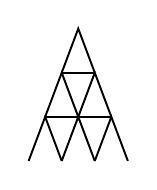
\begin{tikzpicture}[x=4.2mm,y=5.6mm,line width=.7pt]
  \foreach \r in {0,1,2}{
    \pgfmathtruncatemacro{\k}{3-\r}
    \foreach \i in {1,...,\k}{\draw (\i-1+\r/2,\r) -- (\i-.5+\r/2,\r+1) -- (\i+\r/2,\r);}
    \ifnum\k>1 \draw (.5+\r/2,\r+1) -- (\k-.5+\r/2,\r+1);\fi}
\end{tikzpicture}
\end{minipage}
\begin{enumerate}
  \item Controleer dat $u_n = \dfrac{n(3n+1)}{2}$ klopt voor deze drie termen, en bereken $u_{20}$.
  \item Een nieuwe onderste verdieping telt $n$ paar schuine kaarten en $n-1$ platte kaarten. Leid daaruit een recursief voorschrift af.
  \item Hoeveel volledige verdiepingen bouw je met een spel van 52 kaarten?
\end{enumerate}
\begin{solution}
\textbf{a.}~$u_{20}=610$ \quad \textbf{b.}~$u_n=u_{n-1}+3n-1$, $u_1=2$ \quad \textbf{c.}~5
\end{solution}
\begin{fullsolution}
\textbf{a.}~$\tfrac{1\cdot 4}{2}=2$, $\tfrac{2\cdot 7}{2}=7$, $\tfrac{3\cdot 10}{2}=15$, en $u_{20}=\tfrac{20\cdot 61}{2}=610$.\\
\textbf{b.}~Er komen $2n+(n-1)=3n-1$ kaarten bij: $u_n=u_{n-1}+3n-1$ met $u_1=2$.\\
\textbf{c.}~$u_5=40$ en $u_6=57$, dus 5 verdiepingen.
\end{fullsolution}
\end{oefening}

\begin{oefening}[2]
\thema{recursief: terugrekenen}Gegeven: $u_n = 2u_{n-1} + 2$ en $u_4 = 20$. Bereken $u_3$, $u_2$ en $u_1$.
\begin{solution}
9; 3,5; 0,75
\end{solution}
\begin{fullsolution}
Uit $u_n=2u_{n-1}+2$ volgt $u_{n-1}=\dfrac{u_n-2}{2}$. Dus $u_3=\tfrac{18}{2}=9$, $u_2=\tfrac72=3{,}5$ en $u_1=\tfrac{1{,}5}{2}=0{,}75$.
\end{fullsolution}
\end{oefening}

\begin{oefening}[2]
\thema{expliciet: een begin bepaalt geen rij}Gegeven: $u_n = 2^{n-1}$ en $v_n = 2^{n-1} + (n-1)(n-2)(n-3)(n-4)$.
\begin{enumerate}
  \item Bereken van beide rijen de eerste vijf termen.
  \item Iemand zegt: `De rij $1,\ 2,\ 4,\ 8,\ \ldots$ gaat zeker verder met 16.' Wat antwoord je?
\end{enumerate}
\begin{solution}
\textbf{a.}~1, 2, 4, 8, 16 en 1, 2, 4, 8, 40 \quad \textbf{b.}~Niet zeker: de eerste termen leggen de rij niet vast.
\end{solution}
\begin{fullsolution}
\textbf{a.}~Voor $n=1$, 2, 3 en 4 is het product nul, dus beide rijen zijn gelijk. Voor $n=5$ is het product $4\cdot 3\cdot 2\cdot 1=24$, dus $v_5=16+24=40$.\\
\textbf{b.}~Een eindig aantal termen legt de rij niet vast. De puntjes zijn enkel duidelijk als het voorschrift gegeven is of de regelmaat afgesproken is.
\end{fullsolution}
\end{oefening}

\begin{oefening}[2]
\thema{context: recursief}Een zwembad bevat op een maandag 400 g chloor. Elke nacht verdwijnt 20\% van het chloor. Elke ochtend voegt de beheerder 50 g toe. $u_n$ is de hoeveelheid chloor na $n$ dagen.
\begin{enumerate}
  \item Waarom is $u_n = 0{,}8\,u_{n-1} + 50$? Wat is $u_0$?
  \item Bereken $u_1$, $u_2$ en $u_3$.
  \item Bij welke hoeveelheid chloor verandert er niets meer?
\end{enumerate}
\begin{solution}
\textbf{a.}~$u_0=400$ \quad \textbf{b.}~370; 346; 326,8 g \quad \textbf{c.}~250 g
\end{solution}
\begin{fullsolution}
\textbf{a.}~Na het verlies blijft 80\% over, dat is $0{,}8\,u_{n-1}$. Daarna komt er 50 g bij. De beginwaarde is $u_0=400$.\\
\textbf{b.}~$u_1=320+50=370$, $u_2=296+50=346$, $u_3=276{,}8+50=326{,}8$.\\
\textbf{c.}~Er verandert niets als $x=0{,}8\,x+50$, dus $0{,}2\,x=50$ en $x=250$.
\end{fullsolution}
\end{oefening}

\begin{oefening}[2]
\thema{recursief met gevallen}Gegeven: $u_1 = 6$. Is $u_{n-1}$ even, dan is $u_n = \dfrac{u_{n-1}}{2}$. Is $u_{n-1}$ oneven, dan is $u_n = 3u_{n-1} + 1$.
\begin{enumerate}
  \item Schrijf de termen op tot je 1 bereikt. Welk volgnummer heeft die term?
  \item Wat gebeurt er als je daarna verder rekent?
  \item Begin nu met $u_1 = 7$. Welk volgnummer heeft de eerste term 1?
\end{enumerate}
Niemand heeft al kunnen bewijzen dat je vanuit elk natuurlijk getal ooit bij 1 komt.
\begin{solution}
\textbf{a.}~6, 3, 10, 5, 16, 8, 4, 2, 1; volgnummer 9 \quad \textbf{b.}~4, 2, 1 herhaalt zich \quad \textbf{c.}~17
\end{solution}
\begin{fullsolution}
\textbf{a.}~6, 3, 10, 5, 16, 8, 4, 2, 1: de negende term.\\
\textbf{b.}~Na 1 volgt $3\cdot 1+1=4$, en dan 2 en 1: de rij blijft 4, 2, 1 herhalen.\\
\textbf{c.}~7, 22, 11, 34, 17, 52, 26, 13, 40, 20, 10, 5, 16, 8, 4, 2, 1: de zeventiende term.
\end{fullsolution}
\end{oefening}

\begin{oefening}[2]
\thema{context: expliciet en recursief}$u_n$ is het aantal diagonalen van een $n$-hoek. Er geldt $u_3 = 0$, $u_4 = 2$ en $u_5 = 5$.
\begin{enumerate}
  \item Waarom start deze rij niet bij $u_1$?
  \item Leg uit waarom $u_n = \dfrac{n(n-3)}{2}$.
  \item Welke veelhoek heeft 35 diagonalen?
  \item Geef een recursief voorschrift.
\end{enumerate}
\begin{solution}
\textbf{a.}~Een veelhoek heeft minstens 3 hoekpunten \quad \textbf{c.}~een tienhoek \quad \textbf{d.}~$u_n=u_{n-1}+n-2$, $u_3=0$
\end{solution}
\begin{fullsolution}
\textbf{a.}~Een veelhoek heeft minstens 3 hoekpunten.\\
\textbf{b.}~Elk hoekpunt verbind je met alle andere hoekpunten, behalve met zijn twee buren: dat zijn $n-3$ diagonalen per hoekpunt. Zo tel je elke diagonaal twee keer.\\
\textbf{c.}~$n(n-3)=70$ geeft $(n-10)(n+7)=0$, dus $n=10$.\\
\textbf{d.}~$u_{n-1}=\dfrac{(n-1)(n-4)}{2}=\dfrac{n^2-5n+4}{2}$ en $u_n=\dfrac{n^2-3n}{2}$, dus $u_n-u_{n-1}=\dfrac{2n-4}{2}=n-2$.
\end{fullsolution}
\end{oefening}

\begin{oefening}[3]
\thema{periodieke rij}Gegeven: $u_1 = 2$, $u_2 = 3$ en $u_n = \dfrac{u_{n-1}}{u_{n-2}}$ voor $n \geqslant 3$.
\begin{enumerate}
  \item Bereken de eerste acht termen. Wat valt op?
  \item Bereken $u_{100}$.
  \item Toon aan dat hetzelfde gebeurt voor elke $u_1 = a$ en $u_2 = b$ met $a, b \neq 0$.
\end{enumerate}
\begin{solution}
\textbf{a.}~2, 3, $\tfrac32$, $\tfrac12$, $\tfrac13$, $\tfrac23$, 2, 3: om de 6 termen dezelfde \quad \textbf{b.}~$\tfrac12$
\end{solution}
\begin{fullsolution}
\textbf{a.}~$u_3=\tfrac32$, $u_4=\tfrac{3/2}{3}=\tfrac12$, $u_5=\tfrac{1/2}{3/2}=\tfrac13$, $u_6=\tfrac{1/3}{1/2}=\tfrac23$, $u_7=\tfrac{2/3}{1/3}=2$, $u_8=\tfrac{2}{2/3}=3$. Elke term hangt enkel af van de twee vorige, dus vanaf hier herhaalt alles zich om de 6 termen.\\
\textbf{b.}~$100=16\cdot 6+4$, dus $u_{100}=u_4=\tfrac12$.\\
\textbf{c.}~$a,\ b,\ \dfrac{b}{a},\ \dfrac{1}{a},\ \dfrac{1}{b},\ \dfrac{a}{b},\ a,\ b$: na zes termen staan $a$ en $b$ er opnieuw.
\end{fullsolution}
\end{oefening}

\begin{oefening}[3]
\thema{bewijs: voorschrift controleren}Gegeven: $u_1 = 1$ en $u_n = 2u_{n-1} + 1$. Toon aan dat $v_n = 2^n - 1$ aan dit recursieve voorschrift voldoet: controleer de beginterm, en vul $v_{n-1}$ in. Waarom zijn $u_n$ en $v_n$ dan dezelfde rij?
\begin{solution}
Beginterm en stap kloppen, dus de rijen zijn gelijk.
\end{solution}
\begin{fullsolution}
$v_1=2-1=1$ en $2v_{n-1}+1=2\left(2^{n-1}-1\right)+1=2^n-2+1=2^n-1=v_n$.\\
De beginterm en het voorschrift bepalen de rij volledig: uit $u_1$ volgt $u_2$, daaruit $u_3$, enzovoort. Twee rijen met dezelfde beginterm en hetzelfde voorschrift zijn dus gelijk.
\end{fullsolution}
\end{oefening}

\begin{oefening}[3]
\begin{metprent}{bij}
\thema{context: Fibonacci}Bij bijen heeft een mannetje alleen een moeder, en een vrouwtje een moeder en een vader. Vertrek van één mannetje. $u_n$ is het aantal voorouders $n$ generaties terug. Zo is $u_1 = 1$, de moeder, en $u_2 = 2$, haar ouders.
\begin{enumerate}
  \item Bereken $u_3$, $u_4$ en $u_5$.
  \item Leg uit waarom $u_n = u_{n-1} + u_{n-2}$ voor $n \geqslant 3$. Tel daarvoor apart de moeders en de vaders in generatie $n$.
\end{enumerate}
\end{metprent}
\begin{solution}
\textbf{a.}~3, 5, 8
\end{solution}
\begin{fullsolution}
\textbf{a.}~Generatie 2 telt 1 vrouwtje en 1 mannetje. Het vrouwtje heeft 2 ouders en het mannetje 1, dus $u_3=3$: 2 vrouwtjes en 1 mannetje. Zo vind je ook $u_4=2\cdot 2+1=5$: 3 vrouwtjes en 2 mannetjes, en $u_5=2\cdot 3+2=8$.\\
\textbf{b.}~Elke bij in generatie $n-1$ heeft één moeder, dus generatie $n$ telt $u_{n-1}$ vrouwtjes. Alleen de vrouwtjes in generatie $n-1$ hebben een vader. Dat aantal vrouwtjes is $u_{n-2}$, volgens dezelfde redenering. Samen: $u_n=u_{n-1}+u_{n-2}$.
\end{fullsolution}
\end{oefening}

\begin{oefening}[3]
\thema{bewijs: expliciet en recursief}Toon aan dat de rij $u_n = \dfrac{1}{n}$ voldoet aan $u_n = \dfrac{u_{n-1}}{1 + u_{n-1}}$ voor $n \geqslant 2$.
\begin{solution}
Vul $u_{n-1}=\dfrac{1}{n-1}$ in; dat geeft $\dfrac1n$.
\end{solution}
\begin{fullsolution}
$\dfrac{u_{n-1}}{1+u_{n-1}}=\dfrac{\dfrac{1}{n-1}}{1+\dfrac{1}{n-1}}=\dfrac{\dfrac{1}{n-1}}{\dfrac{n}{n-1}}=\dfrac{1}{n}=u_n$.
\end{fullsolution}
\end{oefening}

\begin{oefening}[3]
\thema{hulprij}Gegeven: $u_1 = k$ en $u_n = 2u_{n-1} - 3$.
\begin{enumerate}
  \item Voor welke $k$ is de rij constant?
  \item Neem $k = 5$ en stel $v_n = u_n - 3$. Toon aan dat $v_n = 2v_{n-1}$.
  \item Geef een expliciet voorschrift van $u_n$ voor $k = 5$.
\end{enumerate}
\begin{solution}
\textbf{a.}~$k=3$ \quad \textbf{c.}~$u_n=2^n+3$
\end{solution}
\begin{fullsolution}
\textbf{a.}~Constant betekent $u_2=u_1$, dus $k=2k-3$ en $k=3$. Dan blijft elke term 3.\\
\textbf{b.}~$v_n=u_n-3=2u_{n-1}-3-3=2(u_{n-1}-3)=2v_{n-1}$.\\
\textbf{c.}~$v_1=5-3=2$ en elke term van $v_n$ is het dubbele van de vorige, dus $v_n=2^n$. Dan is $u_n=v_n+3=2^n+3$. Controle: 5, 7, 11, 19.
\end{fullsolution}
\end{oefening}

\begin{oefening}[3]
\thema{Fibonacci: vermoeden en bewijs}Neem de rij van Fibonacci $1,\ 1,\ 2,\ 3,\ 5,\ 8,\ \ldots$ en stel $w_n = u_{n+1} \cdot u_{n-1} - u_n^{\,2}$.
\begin{enumerate}
  \item Bereken $w_2$, $w_3$, $w_4$ en $w_5$. Wat vermoed je?
  \item Toon aan: $w_{n+1} = -w_n$. Vervang daarvoor in $w_{n+1}$ eerst $u_{n+2}$ door $u_{n+1} + u_n$.
\end{enumerate}
\begin{solution}
\textbf{a.}~$1,\ {-1},\ 1,\ {-1}$: vermoeden $w_n=(-1)^n$
\end{solution}
\begin{fullsolution}
\textbf{a.}~$w_2=2\cdot 1-1=1$, $w_3=3\cdot 1-4=-1$, $w_4=5\cdot 2-9=1$, $w_5=8\cdot 3-25=-1$.\\
\textbf{b.}~$w_{n+1}=u_{n+2}u_n-u_{n+1}^{\,2}=(u_{n+1}+u_n)u_n-u_{n+1}^{\,2}=u_n^{\,2}+u_{n+1}(u_n-u_{n+1})$.\\
Omdat $u_{n+1}=u_n+u_{n-1}$ is $u_n-u_{n+1}=-u_{n-1}$. Dus $w_{n+1}=u_n^{\,2}-u_{n+1}u_{n-1}=-w_n$.
\end{fullsolution}
\end{oefening}
\end{oefeningen}

%----------------------------------------------------------------------------------------
% KOPPEL: verbanden met andere leerstof
%----------------------------------------------------------------------------------------
\opdrachtsectie{Koppel}

\lkr{Rationale functies, goniometrie en matrices zijn gezien in het 5de jaar. Telproblemen en logica staan ook in het 6de jaar: kijk na of ze al aan bod kwamen, of laat die twee oefeningen weg.}

\begin{oefeningen}
\begin{oefening}[2]
\koppel{analyse}{Rationale functies} Gegeven: $f(x) = \dfrac{x+1}{x-3}$ en $u_n = f(n)$.
\begin{enumerate}
  \item Bepaal het domein van $f$.
  \item Bereken $u_1$, $u_2$, $u_4$, $u_5$ en $u_6$. Waarom ontbreekt $u_3$?
  \item Hoe los je dat op, zodat er een rij ontstaat met losse termen zonder gat?
\end{enumerate}
\begin{solution}
\textbf{a.}~$\mathbb{R}\setminus\{3\}$ \quad \textbf{b.}~$-1$, $-3$, 5, 3, $\tfrac73$ \quad \textbf{c.}~Start bij $n=4$.
\end{solution}
\begin{fullsolution}
\textbf{a.}~De noemer is nul bij $x=3$.\\
\textbf{b.}~$\tfrac{2}{-2}=-1$, $\tfrac{3}{-1}=-3$, $\tfrac51=5$, $\tfrac62=3$, $\tfrac73$. De term $u_3$ bestaat niet omdat 3 niet in het domein ligt.\\
\textbf{c.}~Neem de rij pas vanaf $n=4$, dus met domein $\{4,5,6,\ldots\}$.
\end{fullsolution}
\end{oefening}

\begin{oefening}[2]
\koppel{analyse}{Goniometrische functies} Gegeven: $u_n = \cos\left(n \cdot \dfrac{\pi}{3}\right)$.
\begin{enumerate}
  \item Bereken de eerste zeven termen. Om de hoeveel termen herhaalt de rij zich?
  \item Wat is de periode van de functie $f(x) = \cos\left(x \cdot \dfrac{\pi}{3}\right)$? Waarom is dat hetzelfde getal?
  \item Schrijf $(-1)^n$ als een cosinus van een veelvoud van $n$.
\end{enumerate}
\begin{solution}
\textbf{a.}~$\tfrac12$, $-\tfrac12$, $-1$, $-\tfrac12$, $\tfrac12$, 1, $\tfrac12$; om de 6 \quad \textbf{b.}~6 \quad \textbf{c.}~$\cos(n\pi)$
\end{solution}
\begin{fullsolution}
\textbf{a.}~De hoeken zijn $\tfrac{\pi}{3},\ \tfrac{2\pi}{3},\ \pi,\ \tfrac{4\pi}{3},\ \tfrac{5\pi}{3},\ 2\pi,\ \tfrac{7\pi}{3}$. Vanaf daar herhaalt de cosinus zich.\\
\textbf{b.}~De periode is $\dfrac{2\pi}{\pi/3}=6$. De rij neemt de functiewaarden in de gehele getallen, en de periode is hier zelf een geheel getal.\\
\textbf{c.}~$\cos(n\pi)$ is $-1$ bij oneven $n$ en 1 bij even $n$.
\end{fullsolution}
\end{oefening}

\begin{oefening}[2]
\koppel{algebra}{Matrices} Gegeven: $A = \begin{pmatrix} 1 & 1 \\ 1 & 0 \end{pmatrix}$.
\begin{enumerate}
  \item Bereken $A^2$, $A^3$ en $A^4$. Welke rij herken je in de elementen?
  \item Toon aan: $A \begin{pmatrix} u_{n-1} \\ u_{n-2} \end{pmatrix} = \begin{pmatrix} u_n \\ u_{n-1} \end{pmatrix}$ is precies het voorschrift van die rij.
\end{enumerate}
\begin{solution}
\textbf{a.}~$\begin{pmatrix} 2 & 1 \\ 1 & 1 \end{pmatrix}$, $\begin{pmatrix} 3 & 2 \\ 2 & 1 \end{pmatrix}$, $\begin{pmatrix} 5 & 3 \\ 3 & 2 \end{pmatrix}$; de rij van Fibonacci
\end{solution}
\begin{fullsolution}
\textbf{a.}~$A^2=\begin{pmatrix} 2 & 1 \\ 1 & 1 \end{pmatrix}$, $A^3=\begin{pmatrix} 3 & 2 \\ 2 & 1 \end{pmatrix}$, $A^4=\begin{pmatrix} 5 & 3 \\ 3 & 2 \end{pmatrix}$. De elementen zijn termen van de rij van Fibonacci.\\
\textbf{b.}~Het product is $\begin{pmatrix} u_{n-1}+u_{n-2} \\ u_{n-1} \end{pmatrix}$. De eerste rij zegt $u_n=u_{n-1}+u_{n-2}$. De tweede rij zegt alleen dat $u_{n-1}$ gelijk blijft aan zichzelf.
\end{fullsolution}
\end{oefening}

\begin{oefening}[2]
\koppel{discreet}{Telproblemen} $u_n$ is het aantal manieren om $n$ verschillende boeken naast elkaar te zetten.
\begin{enumerate}
  \item Bereken $u_1$, $u_2$ en $u_3$.
  \item Leg uit waarom $u_n = n \cdot u_{n-1}$. Denk aan de plaatsen voor het laatste boek.
  \item Bereken $u_6$. Hoe noteren we $u_n$ met een speciaal symbool?
\end{enumerate}
\begin{solution}
\textbf{a.}~1, 2, 6 \quad \textbf{c.}~720; $u_n=n!$
\end{solution}
\begin{fullsolution}
\textbf{a.}~Eén boek: 1 manier. Twee boeken: 2 manieren. Drie boeken: 6 manieren.\\
\textbf{b.}~Zet eerst $n-1$ boeken: dat kan op $u_{n-1}$ manieren. Het laatste boek kan dan op $n$ plaatsen: vooraan, achteraan of ertussen.\\
\textbf{c.}~$u_4=24$, $u_5=120$, $u_6=720$. Dit is de faculteit: $u_n=n!$.
\end{fullsolution}
\end{oefening}

\begin{oefening}[2]
\koppel{discreet}{Logica en bewijzen} Gegeven: $u_n = n^2 + n + 41$.
\begin{enumerate}
  \item Bereken $u_1$, $u_2$, $u_3$ en $u_4$. Wat valt op?
  \item Iemand besluit: `Alle termen van deze rij zijn priemgetallen.' Weerleg dit met een tegenvoorbeeld. Bekijk daarvoor $u_{41}$ zonder rekenmachine.
\end{enumerate}
\begin{solution}
\textbf{a.}~43, 47, 53, 61: priemgetallen \quad \textbf{b.}~$u_{41}=41\cdot 43$
\end{solution}
\begin{fullsolution}
\textbf{a.}~43, 47, 53 en 61 zijn allemaal priemgetallen.\\
\textbf{b.}~$u_{41}=41^2+41+41=41(41+1+1)=41\cdot 43$: geen priemgetal. Enkele voorbeelden bewijzen dus niets, één tegenvoorbeeld weerlegt wel.
\end{fullsolution}
\end{oefening}
\end{oefeningen}

%----------------------------------------------------------------------------------------
\opdrachtsectie{Test jezelf}

\begin{oefeningen}
\begin{oefening}[1]\label{oef:h1-t1}
Gegeven is de rij $5,\ 1,\ 8,\ 1,\ 3$. Wat is $u_3$? Welk volgnummer heeft de term 3? Voor welke volgnummers is $u_n = 1$?
\begin{solution}
8; 5; $n=2$ of $n=4$
\end{solution}
\begin{fullsolution}
De derde term is 8. Het getal 3 staat op plaats 5. Het getal 1 staat op plaats 2 en plaats 4.
\end{fullsolution}
\end{oefening}

\begin{oefening}[1]\label{oef:h1-t2}
Bepaal de eerste vier termen van $u_n = (-1)^n \cdot (n+2)$.
\begin{solution}
$-3,\ 4,\ {-5},\ 6$
\end{solution}
\begin{fullsolution}
$(-1)^1\cdot 3=-3$, $(-1)^2\cdot 4=4$, $(-1)^3\cdot 5=-5$, $(-1)^4\cdot 6=6$.
\end{fullsolution}
\end{oefening}

\begin{oefening}[2]\label{oef:h1-t3}
Bepaal een expliciet voorschrift.
\begin{reeks}[2]
  \item $4,\ 7,\ 10,\ 13,\ \ldots$
  \item $\tfrac13,\ {-\tfrac24},\ \tfrac35,\ {-\tfrac46},\ \ldots$
\end{reeks}
\begin{solution}
\textbf{a.}~$u_n=3n+1$ \quad \textbf{b.}~$u_n=(-1)^{n+1}\cdot\dfrac{n}{n+2}$
\end{solution}
\begin{fullsolution}
\textbf{a.}~Telkens 3 meer: vergelijk met $3n$. Elke term is 1 meer, dus $u_n=3n+1$.\\
\textbf{b.}~Positief bij oneven $n$, teller $n$, noemer $n+2$.
\end{fullsolution}
\end{oefening}

\begin{oefening}[1]\label{oef:h1-t4}
Gegeven: $u_n = n^2 - n$. Is 56 een term van de rij? En 60?
\begin{solution}
56 is de 8ste term; 60 is geen term.
\end{solution}
\begin{fullsolution}
$n^2-n-56=0$ geeft $(n-8)(n+7)=0$, dus $n=8$. $n^2-n-60=0$ geeft $n=\dfrac{1\pm\sqrt{241}}{2}$, dus $n\approx 8{,}26$ of $n\approx -7{,}26$: geen volgnummer.
\end{fullsolution}
\end{oefening}

\begin{oefening}[1]\label{oef:h1-t5}
Gegeven: $u_1 = 4$, $u_2 = 1$ en $u_n = u_{n-1} + 2u_{n-2}$ voor $n \geqslant 3$. Bepaal de eerste vijf termen.
\begin{solution}
4, 1, 9, 11, 29
\end{solution}
\begin{fullsolution}
$u_3=1+8=9$, $u_4=9+2=11$, $u_5=11+18=29$.
\end{fullsolution}
\end{oefening}

\begin{oefening}[2]\label{oef:h1-t6}
Bepaal een recursief voorschrift van $5,\ 6,\ 8,\ 11,\ 15,\ \ldots$
\begin{solution}
$u_n=u_{n-1}+(n-1)$, $u_1=5$
\end{solution}
\begin{fullsolution}
Er komt 1, 2, 3, 4 bij: bij de stap naar $u_n$ is dat $n-1$. Dus $u_n=u_{n-1}+(n-1)$ met $u_1=5$.
\end{fullsolution}
\end{oefening}

\begin{oefening}[2]\label{oef:h1-t7}
Gegeven: $u_n = n^2 + 2n$. Bepaal een recursief voorschrift.
\begin{solution}
$u_n=u_{n-1}+2n+1$, $u_1=3$
\end{solution}
\begin{fullsolution}
$u_{n-1}=(n-1)^2+2(n-1)=n^2-1$, dus $u_n-u_{n-1}=2n+1$. Verder is $u_1=3$. Controle: $u_2=3+5=8=4+4$.
\end{fullsolution}
\end{oefening}

\begin{oefening}[1]\label{oef:h1-t8}
Teken de grafiek van $u_n = (-1)^n \cdot 2n$ voor $n = 1$ tot en met 5. Waarom verbind je de punten niet?
\begin{solution}
$(1,\ {-2})$, $(2,\ 4)$, $(3,\ {-6})$, $(4,\ 8)$, $(5,\ {-10})$; tussen de volgnummers is er geen term.
\end{solution}
\begin{fullsolution}
De termen zijn $-2,\ 4,\ {-6},\ 8,\ {-10}$. Zet de punten los uit. Een rij heeft enkel termen bij natuurlijke volgnummers: tussen $n=1$ en $n=2$ is er niets.
\end{fullsolution}
\end{oefening}

\begin{oefening}[2]\label{oef:h1-t9}
Gegeven is de rij $20,\ 17,\ 14,\ \ldots$ Geef een expliciet voorschrift als de eerste term $u_1$ heet, en als hij $u_0$ heet.
\begin{solution}
$u_n=23-3n$; $u_n=20-3n$
\end{solution}
\begin{fullsolution}
Telkens 3 minder. Met $u_1=20$: $u_n=23-3n$. Met $u_0=20$: $u_n=20-3n$.
\end{fullsolution}
\end{oefening}
\end{oefeningen}

\herhaalschema{%
  \fv{oef:h1-t1}{vb:h1-maanden}{oef:h1-termen}%
  \fv{oef:h1-t2}{vb:h1-termen}{oef:h1-expl}%
  \fv{oef:h1-t3}{vb:h1-opstellen}{oef:h1-opstellen}%
  \fv{oef:h1-t4}{vb:h1-isterm}{oef:h1-isterm}%
  \fv{oef:h1-t5}{vb:h1-twee}{oef:h1-recterm}%
  \fv{oef:h1-t6}{vb:h1-recopst}{oef:h1-recopst}%
  \fv{oef:h1-t7}{vb:h1-omzet}{oef:h1-omzet}%
  \fv{oef:h1-t8}{vb:h1-grafiek}{oef:h1-grafiek}%
  \fv{oef:h1-t9}{vb:h1-nul}{oef:h1-nuleen}}

\ifzelfstudie
\section*{Maak je eigen samenvatting}
Sluit dit boek en schrijf in je schrift: wat is een term, een volgnummer en de algemene term, wat is het verschil tussen een expliciet en een recursief voorschrift, hoe stel je ze op, hoe test je of een getal een term is, wanneer start je bij $u_0$, hoe ziet de grafiek van een rij eruit, en welke fouten wil je vermijden? Vergelijk daarna met de kaders.
\fi
